\chapter{Marco teórico}
\label{marco}

Desde tiempos inmemorables las imágenes han acompañado al ser humano, desde las
pinturas rupestres en la Cueva de Altamira, pasando por los códices Mayas, los
daguerrotipos, las cámaras \textit{Pinhole} o los rayos X de Röntgen hasta las
imágenes del Curiosity Rover de la NASA. En este capítulo se introducen
conceptos básicos sobre las imágenes digitales, su procesamiento y su utilidad
en la lucha contra el cáncer de mama. También se abordan ideas expuestas en
trabajos similares.

\section{Breve introducción a las imágenes digitales}

Hay muchos tipos de imágenes digitales, en esta tesis nos enfocaremos en las
mamografías. Las imágenes digitales están formadas por una unidad básica
llamada \textit{pixel}. Una computadora representa una imagen como un arreglo
bidimensional de píxeles, cada posición de ese arreglo almacena valores
numéricos. Con el fin de conocer la posición de un pixel las imágenes tienen un
\textit{sistema de coordenadas}. A diferencia del sistema cartesiano, el origen
está en la parte superior izquierda (Figura \ref{fig:coordinates}). 

\shorthandoff{>} % hack to combine tikZ and Spanish
    % TikZ picture with origin upper left
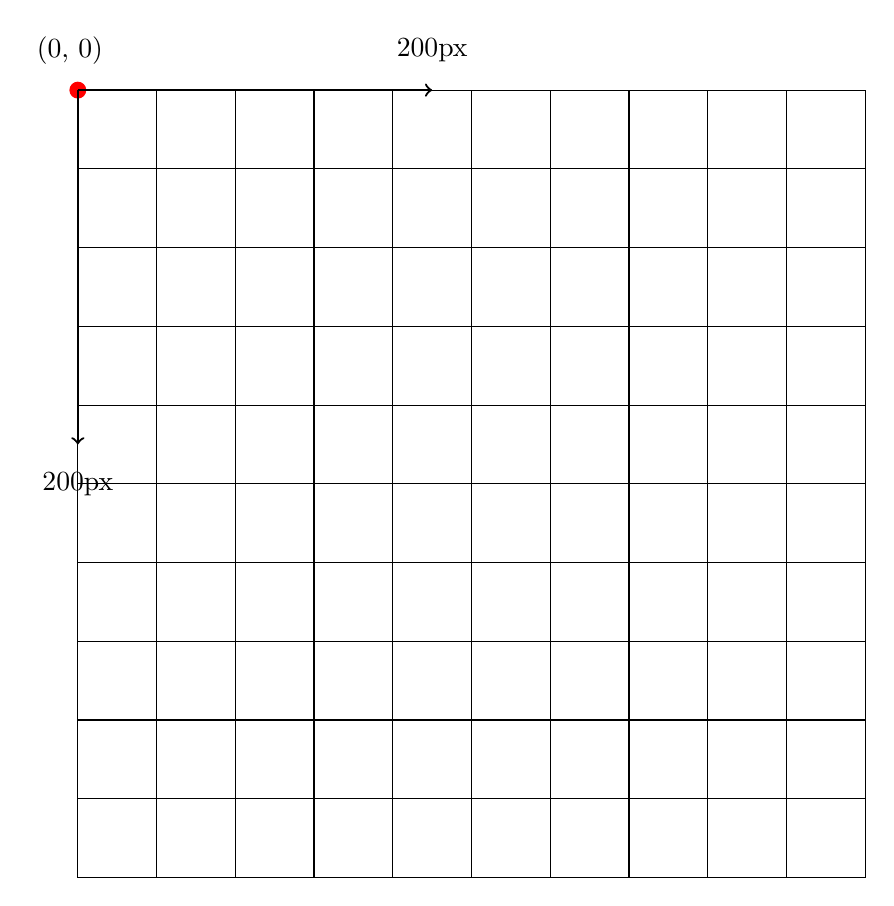
\begin{tikzpicture}[yscale=-1] 
    % 10x10 grid
    \draw (0, 0) grid (10, 10);
    % origin point
    \draw [color=red, fill=red] (0, 0) circle (0.1);
    % x-axis
    \draw [thick,->] (0, 0) -- (4.5, 0);
    % y-axis
    \draw [thick,->] (0, 0) -- (0, 4.5);
    % origin label
    \node at (-0.1, -0.5) {(0, 0)};
    % x-axis label
    \node at (4.5, -0.5) {200px};
    % y-axis label
\node at (0, 5) {200px};
\end{tikzpicture}

\shorthandon{>} 

% Improve explanation about light and discrete values 
La \textit{adquisición de imágenes} es el proceso por el cual una escena se
convierte en un arreglo de píxeles. El primer paso de este proceso se conoce
como \textbf{muestreo} y consiste en la conversión de una distribución continua
de luz a su representación discreta. El segundo paso es la
\textit{cuantificación}, que consiste en la conversión a una escala de enteros.
De acuerdo a lo anterior, una imagen también puede definirse como una función
discreta como se muestra en la Ecuación \ref{eq:discretized}. 

% nota al pie sobre matlab o poner otra ecuación

\begin{equation}
\label{eq:discretized}
    \begin{split}
            f(x,y) & = 
            \begin{pmatrix}
                f(1,1) & f(1,2) & \cdots & f(1,y) \\
                f(2,1) & f(2,2) & \cdots & f(2,y) \\
                \vdots & \vdots & \ddots & \vdots \\
                f(x,1) & f(x,2) & \cdots & f(x,y) \\
            \end{pmatrix}
    \end{split}
\end{equation}

\begin{table}
  \caption[Escala de grises]{Escalas de grises \cite{burger2008digital}} 
  \label{table:grayscales}
\begin{center}
{\small
    \begin{tabular}{c|c|c}
    \hline
    {\bf Bits por pixel} & 
    {\bf Rango} & 
    {\bf Uso} \\
    \hline
    1  & 0\dots1     & Imágenes binarias: documentos, fax \\
    8  & 0\dots255   & Universal: Fotos, escaneos, impresiones   \\
    12 & 0\dots4095  & Alta calidad: Fotos, escaneos, impresiones   \\
    14 & 0\dots16383 & Profesional: Fotos, escaneos, impresiones   \\
    16 & 0\dots65535 & Altísima calidad: Medicina, astronomía   \\
    \hline
    \end{tabular}
}
\end{center}
\end{table}

En las imágenes \textit{a color} cada pixel generalmente tiene tres canales, es
decir, cada pixel almacena una tripleta de valores, las imágenes \textit{en
escala de grises} en cambio tienen un sólo canal por pixel. El rango de valores
que puede tomar cada pixel es conocido como \textit{bit de profundidad}. Cada
pixel puede almacenar $2^k$ valores diferentes que son números enteros en el
rango: $[0\dots2^k - 1]$ donde $0$ es representa el color negro y $2^k$ el color
blanco el blanco. La Tabla \ref{table:grayscales} sumariza información sobre
las imágenes en escala de grises y en la Figura \ref{grayscales} podemos ver la
misma imagen con diferentes niveles de grises.

\begin{figure}[h]
    \centering

    \subfloat[150 dpi]{\includegraphics[height=40mm]{images/dpi150.jpg}}
    \subfloat[125 dpi]{\includegraphics[height=40mm]{images/dpi125.jpg}}
    \subfloat[100 dpi]{\includegraphics[height=40mm]{images/dpi100.jpg}}
    \subfloat[75 dpi]{\includegraphics[height=40mm]{images/dpi75.jpg}}

    \bigskip

    \subfloat[50 dpi]{\includegraphics[height=40mm]{images/dpi50.jpg}}
    \subfloat[25 dpi]{\includegraphics[height=40mm]{images/dpi25.jpg}}
    \subfloat[10 dpi]{\includegraphics[height=40mm]{images/dpi10.jpg}}
    \subfloat[5 dpi]{\includegraphics[height=40mm]{images/dpi5.jpg}}

  \caption{La imagen de Lenna obtenida de \textit{The USC-SIPI Image Database}
  vista con distintos distintos valores dpi}
  
  \label{grayscales}
\end{figure}

Otros término básico para entender una imagen es la \textit{resolución}, la
resolución de una imagen especifica las dimensiones espaciales de la imagen en
el mundo real y es dada por el número de elementos de la imagen por medida; por
ejemlo, \textit{puntos por pixel}, (dpi, por sus siglas en inglés). En la
Figura \ref{resolution} podemos ver la misma imagen con diferente resolución.

\begin{figure}[h]
    \centering

    \subfloat[256 niveles de grises]{\includegraphics[height=40mm]{images/lenna256.jpg}}
    \subfloat[128 niveles de grises]{\includegraphics[height=40mm]{images/lenna128.jpg}}
    \subfloat[64 niveles de grises]{\includegraphics[height=40mm]{images/lenna64.jpg}}
    \subfloat[32 niveles de grises]{\includegraphics[height=40mm]{images/lenna32.jpg}}

    \bigskip

    \subfloat[16 niveles de grises]{\includegraphics[height=40mm]{images/lenna16.jpg}}
    \subfloat[8 niveles de grises]{\includegraphics[height=40mm]{images/lenna8.jpg}}
    \subfloat[4 niveles de grises]{\includegraphics[height=40mm]{images/lenna4.jpg}}
    \subfloat[2 niveles de grises]{\includegraphics[height=40mm]{images/lenna2.jpg}}

  \caption{Diferentes resoluciones. Imagen de Lenna obtenida de
  \textit{The USC-SIPI Image Database}}
  
  \label{resolution}
\end{figure}

\section{Introducción al procesamiento de imágenes}

El \textit{procesamiento de imágenes} es el conjunto de técnicas y algoritmos
utilizados con un propósito doble: mejorar la apariencia visual de las imágenes
al observador humano y preparar las imágenes para la medición de sus
estructuras y características.

La modificación de \textit{histogramas} es un recurso muy utilizado para evaluar

Un histograma es una distribución de frecuencia, el histograma de una imagen
describe la frecuencia y la intensidad de valores que ocurren en una imagen
\cite{burger2008digital}. Está demostrado que la ecualización de histogramas es
un método efectivo para mejorar la calidad de las imágenes médicas.

\begin{figure}[h]
    \centering

    \subfloat[Bajo contraste\label{hist:a}]{\includegraphics[height=40mm]{images/rightskewed.jpg}}
    \subfloat[Contraste normal\label{hist:b}]{\includegraphics[height=40mm]{images/mandril.jpg}}
    \subfloat[Alto contraste\label{hist:c}]{\includegraphics[height=40mm]{images/leftskewed.jpg}}

    \bigskip

    \subfloat[Histograma de \protect\subref{hist:a}]{\includegraphics[height=40mm]{images/histogram-right.jpg}}
    \subfloat[Histograma de \protect\subref{hist:b}]{\includegraphics[height=40mm]{images/histogram-mandril.jpg}}
    \subfloat[Histograma de \protect\subref{hist:c}]{\includegraphics[height=40mm]{images/histogram-left.jpg}}

  \caption{La misma imagen con diferentes contrastes y su respectivo histograma. En \protect\subref{hist:a} se visualiza la imagen con un bajo contraste.
  Imagen del Mandril obtenida de \textit{The USC-SIPI Image Database}}
  
  \label{fig:histograms}
\end{figure}

\section{Imágenes médicas}

% cross-sectional -> cortes transversales
Uno de los usos más importantes de las imágenes digitales recae en la medicina,
existe una gran variedad de imágenes médicas. Podemos mencionar las
\textbf{tomografías computarizadas} que son imágenes del corte transversal de
alguna parte del cuerpo, son generadas con rayos X. Las \textbf{resonancias
magnéticas} son generadas a partir de la propiedades magnéticas de un tejido.
La teoría sobre la cual descansa la generación de imágenes de este tipos está
ligada a la teoría especial de la relatividad y la mecánica cuántica. Los
\textbf{ultrasonidos} son generados a partir de ondas acústicas, su uso no es
exclusivo de la medicina, también son usados en la sismología, el estudio de
grietas microscópicas o en el estudio del fondo del mar. Las imágenes generadas
por la \textbf{medicina nuclear} se valen del uso de isótopos radioactivos. Por
último tenemos las \textbf{radiografías} (las mamografías son radiografías)
\cite{suetens2009fundamentals}.

\begin{figure}[h]
    \centering

    \subfloat[Tomografía]{\includegraphics[height=40mm]{images/computed-tomography.png}}
    \hspace{1cm}
    \subfloat[Resonancia magnética]{\includegraphics[height=40mm]{images/computed-tomography.png}}
    \hspace{1cm}
    \subfloat[Ultrasonido]{\includegraphics[height=40mm]{images/computed-tomography.png}}

    \bigskip

    \subfloat[Medicina nuclear]{\includegraphics[height=40mm]{images/computed-tomography.png}}
    \hspace{1cm}
    \subfloat[Radiografía]{\includegraphics[height=40mm]{images/computed-tomography.png}}

  \caption{Diferentes imágenes médicas obtenidas de \textit{The Cancer Imaging Archive}}
  
  \label{medicalimages}
\end{figure}

\subsection{Mamografías}

El \textit{cáncer de mama} es un padecimiento en el que se desarrollan células
malignas en los tejidos de la mama, estas se duplican cada 100-300 días, un
tumor de 1 cm ha realizado alrededor de treinta duplicaciones antes de alcanzar
este tamaño, lo que implica que el cáncer de mama tiene, como mínimo, unos
siete años de evolución. Tomando en cuenta lo anterior se entiende la
importancia de la detección prematura de esta enfermedad \cite{mxcancer}.

Cada estudio mamográfico tiene cuatro imágenes. Figura \ref{fig:views}.

\begin{figure}[h]
    \centering

    \subfloat[Craniocaudal derecha]{\includegraphics[height=40mm]{images/computed-tomography.png}}
    \hspace{1cm}
    \subfloat[Craniocaudal izquierda]{\includegraphics[height=40mm]{images/computed-tomography.png}}

    \bigskip

    \subfloat[Mediolateral oblicua]{\includegraphics[height=40mm]{images/computed-tomography.png}}
    \hspace{1cm}
    \subfloat[Mediolateral oblicua]{\includegraphics[height=40mm]{images/computed-tomography.png}}

  \caption{Cuatro vistas en un estudio mamográfico}
  
  \label{fig:views}
\end{figure}


%Las mamografías son exámenes radiográficos diseñados para detectar el cáncer de
%mamá \cite{bushberg2011essential}.

\subsection{Proceso de formación de una mamografía}

Obtener una imagen mamográfica es un desafío debido a que la mama está
constituida por tejidos similares entre sí y porque las lesiones buscadas por
el radiólogo que indicarían la presencia de un tumor son pequeñas o similares
al tejido normal \cite{mxcancer}. Las mamografías son imágenes obtenidas al
exponer la mama a una dosis leve de rayos X. Los mastógrafos disponen de un
receptor que captura ...

%In screening mammography, as practiced in USA, (also in Mexico), two x-ray
%images of each breast, in the medio lateral oblique and craniocaudal views,
%are acquired. 
Los estudios mamográficos más recientes son conocidos como 

\subsection{Estándar DICOM}

DICOM (Digital Imaging and Communication in Medicine) es el estándar en las
imágenes médicas, fue desarrollado por la ACR (American College of Radiology)
en conjunto con NEMA (National Electrical Manufacturers Association)
\cite{acrnema, pianykh2011digital}.  

Mencionar DICOMDIR aquí.

\subsection{Estructura de un archivo DICOM}

Los archivos DICOM son más que un formato ... Mencionar las etiquetas.


\subsection{Lesiones comunes}

%Mammographic features characteristic of breast cancer are masses, particularly
%ones with irregular or “spiculated” margins; clusters of microcalcifications
%(tiny deposits of calcium); and architectural distortions of breast structures. 

Una \textit{masa} es una estructura tridimensional usualmente visible en dos
proyecciones ortogonales. Las {asimetrías} --

\textit{Calcificaciones} y \textit{microcalcificaciones}, que son depósitos de calcio.

\textit{Distorsión de la arquitectura}, 

\subsection{BI-RADS}

BI-RADS (Breast Imaging Reporting and Data System Atlas)
\cite{reston2003birads} provee la terminología básica y un sistema de
clasificación para los estudios mamográficas. Fue creado por la ACR para
estandarizar los reportes de los radiólogos y reducir la confusión en las
interpretaciones. Las categorías de evaluación son:

\begin{enumerate}[a)]
    \item Categoría incompleta
    \begin{enumerate}[i.]
        \item Categoría 0: Necesita evaluación adicional y/o más mamografías para comparar.
    \end{enumerate}
    \item Mammographic assessment complete:
    \begin{enumerate}[i.]
        \item Categoría 1: Negativo.
        \item Categoría 2: Hallazgo(s) benigno(s).
        \item Categoría 3: Hallazgo(s) benignos(s) probable(s).
        \item Categoría 4: Anormalidades sospechosas.
        \item Categoría 5: Highly suggestive of malignancy.         
        \item Categoría 6: Proven malignancy.
    \end{enumerate}
\end{enumerate}

\subsection{Sistemas CAD}

Un sistema CAD (Computer Aided Diagnosis) puede mejorar el desempeño de los
radiólogos en la predicción del cáncer de mama.

\subsection{Preprocesamiento}
El preprocesamiento es la etapa previa al procesamiento de imágenes \textit{per
se}, el principal objetivo de esta etapa es mejorar la calidad de la imagen
para que quede lista para su posterior procesamiento \cite{ponraj2011survey}
que muchas veces son algoritmos para un sistema CAD (Computer Aided Diagnosis).
El preprocesamiento también se utiliza para mejorar la visibilidad del
observador \cite{rahmati2010new}. 

\subsubsection{Preprocesamiento de mamografías}
El preprocesamiento de mamografías es especial porque no es como los otros tipos
de preprocesamiento, hay preprocesamiento específico para mamogramas.

\section{Ruido}

\subsection{Ruido en mamografías}

\cite{hashimoto2008practical}
Noise in digital mammographies (Practical digital mammography by Beverly
Hashimoto) De acuerdo a Hachimoto en las imágenes mamográficas tenemos cuatro
tipos de ruido:

\begin{enumerate}
    \item Ruido cuántico.
    \item fixed electronic
    \item señales secundarías
    \item quanta secundario indirecto
\end{enumerate}

\section{Trabajos relacionados}
% You organize this section by idea, and not by author or by publication

% Other databases
Existen múltiples bases de datos, públicas o privadas, utilizadas en estudios
relacionados a la detección del cáncer de mama. Las características de ellas
son diferentes. En la Tabla \ref{table:overviewdb} se muestran algunas de ellas.

MIAS \cite{sucklingmini} aunque es el recurso más viejo, sigue siendo
ampliamente utilizado. MIAS no tiene soporte actualmente. DDSM
\cite{heath2000digital} es el recurso más utilizado. Es importante notar la
presencia de dos recursos latinoamericanos, más específicamente, brasileños.

IRMA (Image Retrieval in Medical Applications) is a extensive project
\cite{doi:10.1117/12.770325} ...

MIRaCLe (Mammography Image reading for Radiologists and Computers Learning
Database) es un repositorio dinámico para el entrenamiento y evaluación de
computadoras y radiólogos \cite{antoniou2009web}. MIRaCLe cuenta con un sistema
web que provee dos servicios: \textit{Software de Clasificación y Evaluación},
donde el usuario puede realizar consultas, visualizar y escoger diferentes
imágenes para probar algoritmos CAD y el \textit{Evaluación de Radiólogos}, que
provee funcionalidades para evaluar el desempeño de un radiólogo.

MIDAS (Mammographic Image Database for Automated Analysis) es una base de datos
con muestras tomadas entre la población femenina de Brasil
\cite{fernandes2012midas}. De esta base de datos destaca la inclusión de
secuencias de datos genómicas de los pacientes y su apertura a la colaboración
externa, -brand new inovation-. MIDAS cuenta también con un sistema web.

BancoWeb es una base de datos creada por LAPIMO (Laboratório de Análise e
Processamento de Imagens Médicas e Odontológicas) \cite{matheus2011online}.

INbreast: \cite{moreira2012inbreast}, es una base de datos , los autores
sugieren características esenciales de una base de datos que conllevaría a la
creación de sistemas CAD.

Magic-5 \cite{bellotti2004magic} es la evolución de GPCalma (Grid Platform for
Computer Assisted Library for MAmmography) \cite{lauria2006gpcalma}, una base
de datos distribuida. 

La Universidad de Calgary ha creado un banco de imágenes conocido como AMDI
\cite{suri2006recent} cuya función principal es ser un atlas que ayude a los
radiólogos a encontrar casos similares cuando emitir un diagnóstico se torna
complicado. Pero también sirve como un sistema educativo
\cite{guliato2009indiam}.

% Otras bases de datos mencionadas en la literatura son Trueta, LLNL, Málaga, NDMA.

\afterpage{
    \clearpage
\begin{landscape}
%\begin{sidewaystable}
\begin{table}[h]
  \caption{Algunas bases de datos de mamografías digitales} 
  \label{table:overviewdb}
\begin{center}
{\small
    \rowcolors{1}{}{lightgray} 
    \begin{tabular}
    {c| >{\centering\arraybackslash}m{1in} | >{\centering\arraybackslash}m{1in}|c| 
    >{\centering\arraybackslash}m{0.6in} | >{\centering\arraybackslash}m{0.6in} |c|c|c}
    \hline

    {\bf Nombre} & 
    {\bf Número de casos} & 
    {\bf Número de imágenes} & 
    {\bf Proyecciones} & 
    {\bf Tipo de archivo} & 
    {\bf Lugar de origen} & 
    {\bf Año} &
    {\bf ACR} & 
    {\bf BIRADS} \\
    \hline
    mini-MIAS & 161  & 322    & MLO       & PGM   & Reino Unido    & 1994 & yes & yes \\[4ex] 
    DDSM      & 2620 & 10480  & MLO \& CC & LJPEG & Estados Unidos & 1999 & yes & yes \\[4ex] 
    BancoWeb  & 320  & 1'400  & MLO \& CC & TIFF  & Brasil         & 1999 & yes & yes \\[4ex] 
    INbreast  & 115  & 410    & MLO \& CC & DICOM & Portugal       & 2012 & yes & yes \\[4ex] 
    MIDAS     & 100  & 600    & MLO       & DICOM & Brasil         & 2011 & yes & yes \\[4ex] 
    IRMA      & -    & 10'509 & MLO \& CC & LJPEG & Alemania       & 2008 & yes & yes \\[4ex] 
    MIRaCLe   & 196  & 10480  & MLO \& CC & LJPEG & Grecia         & 2009 & yes & yes \\[4ex] 
Magic-5 (GPCalma) & 967  & 3369  & MLO \& CC & DICOM & Italia      & 2002 & no  & yes \\[4ex] 
    \hline
    \end{tabular}
}
\end{center}
\end{table}
%\end{sidewaystable}
\end{landscape}
} % end of afterpage

% Preprocessing related works
Una gran cantidad de trabajos de investigación se han desarrollado en el
campo del preprocesamiento de imágenes mamográficas. En esta sección se revisan
varios enfoques expuestos en la literatura existente, algunos de los cuales se
rescataron en este trabajo para crear un método híbrido que combina las
fortalezas de estos. 

El preprocesamiento de mamogramas engloba algunas tareas también válidas en
el preprocesamiento de otro tipo de imágenes médicas como remoción de ruido,
mejora de contraste o reducción del área de trabajo, no obstante, también
existe el \textit{preprocesamiento orientado a mamografías} que comprende
tareas como orientación de la dirección de la mama, la supresión del músculo
pectoral o la detección del pezón.

%\subsection{Remoción del músculo pectoral}

El trabajo de Maitra utiliza un método híbrido -mixto- de tres fases
\cite{maitra2012technique}. La fase inicial es la mejora de contraste con el
algoritmo CLAHE, después se aisla el músculo pectoral de la región de interés y
finalmente se suprime utilizando el algoritmo \textit{seeding region growing}.
El -enfoque- de Maitra es interesante, pues su método es orientado a
mamografías. Su método pudo aislar el músculo pectoral en la mayoría de las
imágenes de miniMIAS.

Akram también propone la remoción del músculo pectoral además de etiquetas y
artefactos \cite{akram2013preprocessing}. Su propuesta utiliza el método de
contorno activo. 

Por su parte Mirzaalian \cite{mirzaalian2007pre} plantea un algoritmo para la
extracción del contorno de la mama y otro para la extracción del músculo
pectoral. Para extraer el contorno de la mama utiliza en conjunto la
ecualización de histogramas, una técnica de -convolución- con una máscara, que
sirve como un filtro de paso bajo, binarización y -labeling-, 

Otros trabajos como el de Rahmati \cite{rahmati2010new} concentran su atención en
mejorar una sola tarea. Este trabajo propone una versión mejorada de CLAHE:
FCLAHE. Su método trabaja las desventajas de CLAHE, que mejora el -frente- y el
-fondo- linealmente, de tal manera que el resultado es una imagen con alto
contraste al -frente- y en el -fondo-. La mejora del fondo puede conducir a que
los radiólogos identifiquen -falsos positivos-. Para probar la eficiencia del
algoritmo propuesto ejecutan un algoritmo de segmentación sobre imágenes que
fueron pasadas sobre CLAHE y sobre FCLAHE, obteniendo una mejora en el accuracy
de FCLAHE.

% =========[ denoising ]===========

Dos Santos \cite{romualdopre}, \cite{dos2009mammography} propone un método para
reducir el ruido quantum/Poisson, el ruido con más presencia en imágenes mamográficas.
Utiliza la transformada de \textit{Anscombe} en conjunto con el filtro de
Wiener para reducir el ruido, además del filtro Inverso del Dominio de la
Frecuencia para mejorar las imágenes. Dado que el ruido cuántico puede ser
descrito por la distribución de Poisson se utiliza la transformada de Anscombe
para convertir este tipo de ruido en ruido aditivo que es eliminado utilizando
el filtrado Wiener. Su método fue evaluado utilizando un sistema CAD. 

Naveed \cite{naveed2012quantum} propone un método de remoción de ruido dividido
en dos módulos, detección y filtrado de ruido. La detección se lleva a cabo
utilizando redes neuronales y para la remoción del ruido se utilizan tres
filtros, que son \textit{non local mean} (NLM), el filtro adaptativo de Wiener
y el frost filter based methos. La remoción busca preservar los detalles. Este
estudio propone la eliminación del ruido impulsivo y cuántico. Se evalúa el
método comparando la precisión de algoritmos de \textit{clasificación} en
presencia/ausencia de ruido.

% =========[ surveys ]===========

Ponraj y Pisano hacen estudios extensivos del estado del arte del algoritmos
utilizados para modificar imágenes mamográficas \cite{ponraj2011survey},
\cite{pisano2000image}.

La reducción del área de trabajo es estudiada por \cite{holguinpre} y
\cite{dehghani2011method}.


